\subsection{ArrowParallel Implementations}
\begin{frame}[fragile]{Multicore}
\begin{lstlisting}[frame=htrbl]
instance (NFData b, ArrowApply arr, ArrowChoice arr) =>
	ArrowParallel arr a b conf where
		parEvalN _ fs = listApp fs >>>
			arr (flip using $ parList rdeepseq)
\end{lstlisting}
\begin{center}
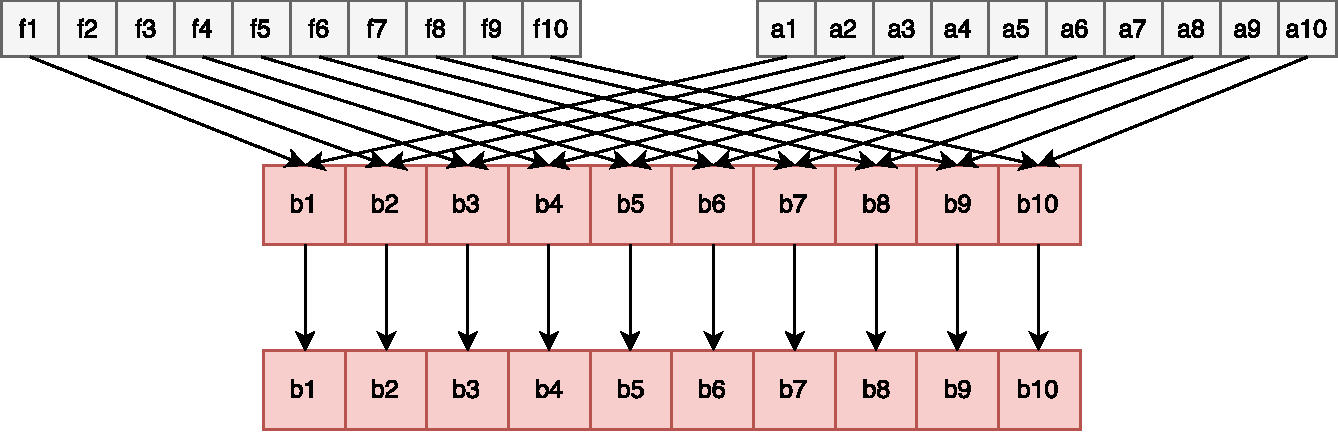
\includegraphics[scale=0.5]{images/parEvalNMulticore}
\end{center}
\end{frame}

\begin{frame}[fragile]{ParMonad}
\begin{lstlisting}[frame=htrbl]
instance (NFData b, ArrowApply arr, ArrowChoice arr) =>
	ArrowParallel arr a b conf where
		parEvalN _ fs = 
			(arr $ \as -> (fs, as)) >>>
			zipWithArr (app >>> arr spawnP) >>>
			...
\end{lstlisting}
\begin{center}
\includegraphics[scale=0.4]{images/parEvalNParMonad1}
\end{center}
\end{frame}

\begin{frame}[fragile]{ParMonad}
\begin{lstlisting}[frame=htrbl]
			...
			arr sequence >>>
			arr (>>= mapM get) >>>
			arr runPar
\end{lstlisting}
\begin{center}
\includegraphics[scale=0.4]{images/parEvalNParMonad2}
\end{center}
\end{frame}


\begin{frame}[fragile]{Eden (1)}
For Eden we need separate implementations.\\~\\
This is because of \code{spawnF}'s
\begin{lstlisting}[frame=htrbl]
spawnF :: (Trans a, Trans b) => [a -> b] -> [a] -> [b]
\end{lstlisting}
and \code{app}'s signature
\begin{lstlisting}[frame=htrbl]
app :: (ArrowApply arr) => arr (arr a b, a) b
\end{lstlisting}
which don't fit together.\\~\\
\pause
Hacky alternative:
\begin{lstlisting}[frame=htrbl]
class (Arrow arr) => ArrowUnwrap arr where
arr a b -> (a -> b)
\end{lstlisting}
\end{frame}

\begin{frame}[fragile]{Eden (2)}
Implementation for Functions
\begin{lstlisting}[frame=htrbl]
instance (Trans a, Trans b) => ArrowParallel (->) a b conf where
	parEvalN _ fs as = spawnF fs as
\end{lstlisting}
\begin{center}
\includegraphics[scale=0.5]{images/parEvalNEden}
\end{center}
\end{frame}

\begin{frame}[fragile]{Eden (3)}
Implementation for the Kleisli Type:
\begin{lstlisting}[frame=htrbl]
instance (Monad m, Trans a, Trans b, Trans (m b)) =>
ArrowParallel (Kleisli m) a b conf where
parEvalN conf fs =
	(arr $ parEvalN conf (map (\(Kleisli f) -> f) fs)) >>>
	(Kleisli $ sequence)
\end{lstlisting}
\begin{center}
\includegraphics[scale=0.5]{images/parEvalNEden}
\end{center}
\end{frame}